We will use GitHub (and GitHub Projects in particular) as the project management tool used to assign tasks, impose deadlines, and track progress.
Email is \href{https://facilethings.com/blog/en/your-email-is-not-a-todo-list}{not a task management tool}.

To start, once the repository for the project is created, you can create a project board by clicking on the Projects tab and then New project.
Project name should be the same as the repository name. 
Add a new column for `Next Up' tasks.
We will have four status: To do, Next Up, In progress, Done.
Here is an example:
\begin{center}
    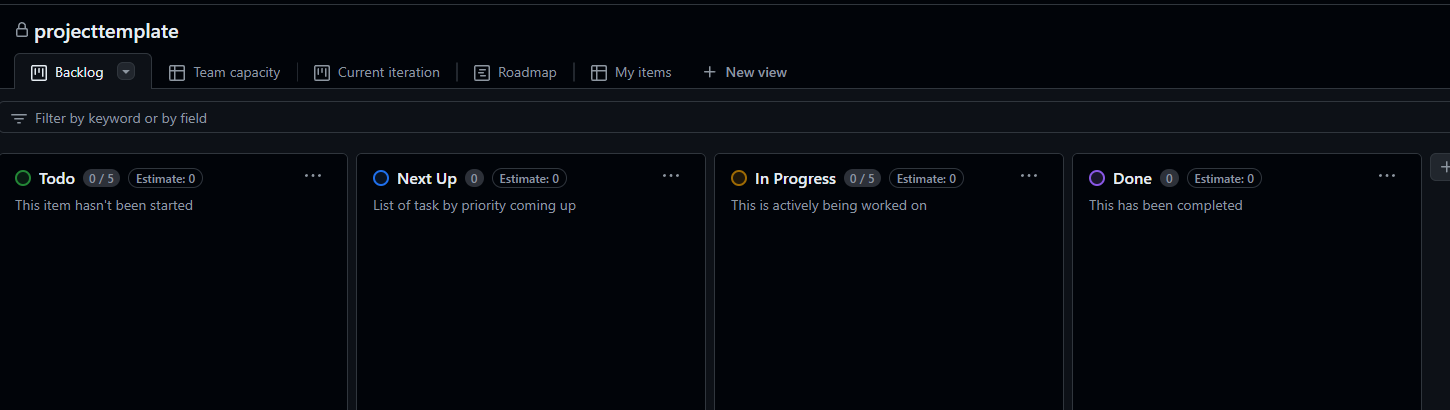
\includegraphics[width=.8\textwidth]{./figures/workflow/gitproject_example1.png}
\end{center}
Then go to `Workflow' in the project, and automate the addition of tasks from the repository to the project. 
To do this, then go to `Auto-add to Project', and Edit the filter to just be `is:issue'. 
New added issues will not be assigned status by default, so you will need to manually assign them to the correct column.

\subsection{Tasks - or Issues}
Tasks are created as issues in the repository.
To create a new issue, click on the Issues tab and then New issue.
\begin{center}
    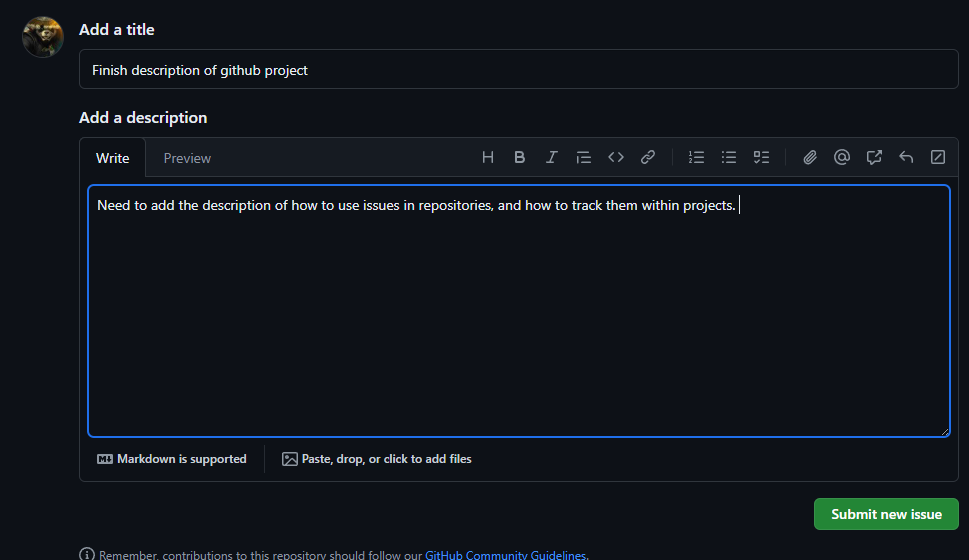
\includegraphics[width=.8\textwidth]{./figures/workflow/gitproject_issue1.png}
\end{center}
Issues should be created \textbf{irrespective} if they are code or non-code tasks.
We can check on the progress of the project by looking at the project board.
Each issue should be assigned to a member of the team, and the issue should be moved to the `In progress' column when work begins.
Issues should be closed when the task is completed.

\begin{center}
    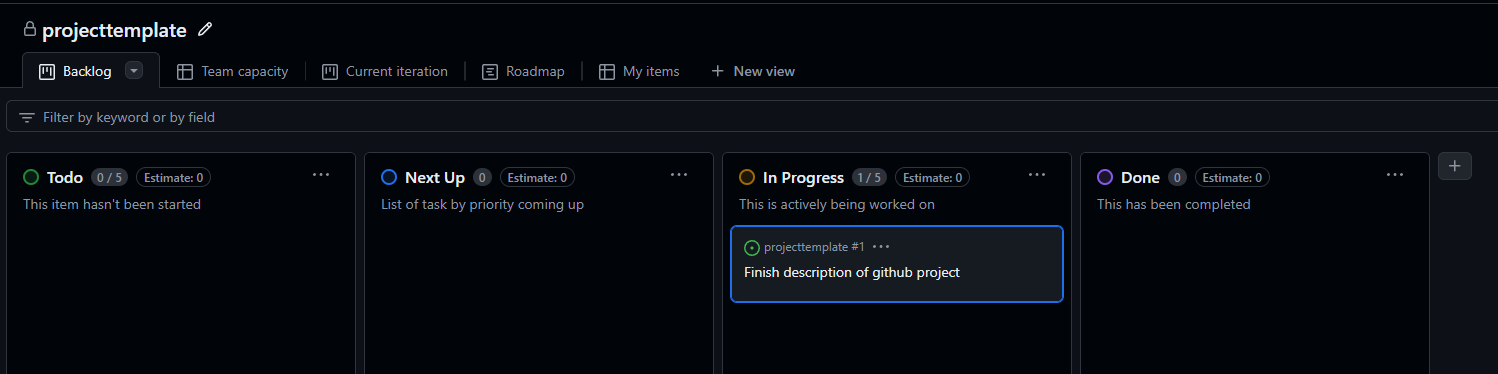
\includegraphics[width=.8\textwidth]{./figures/workflow/gitproject_example2.png}
\end{center}

Also, we can comment on issues to ask for clarification or to provide updates.
We can also assign labels to issues to categorize them.
For example, we can have labels for different types of tasks, such as data cleaning, data analysis, or writing.
We can also have labels for different parts of the project, such as the literature review, the data analysis, or the conclusion.
\begin{center}
    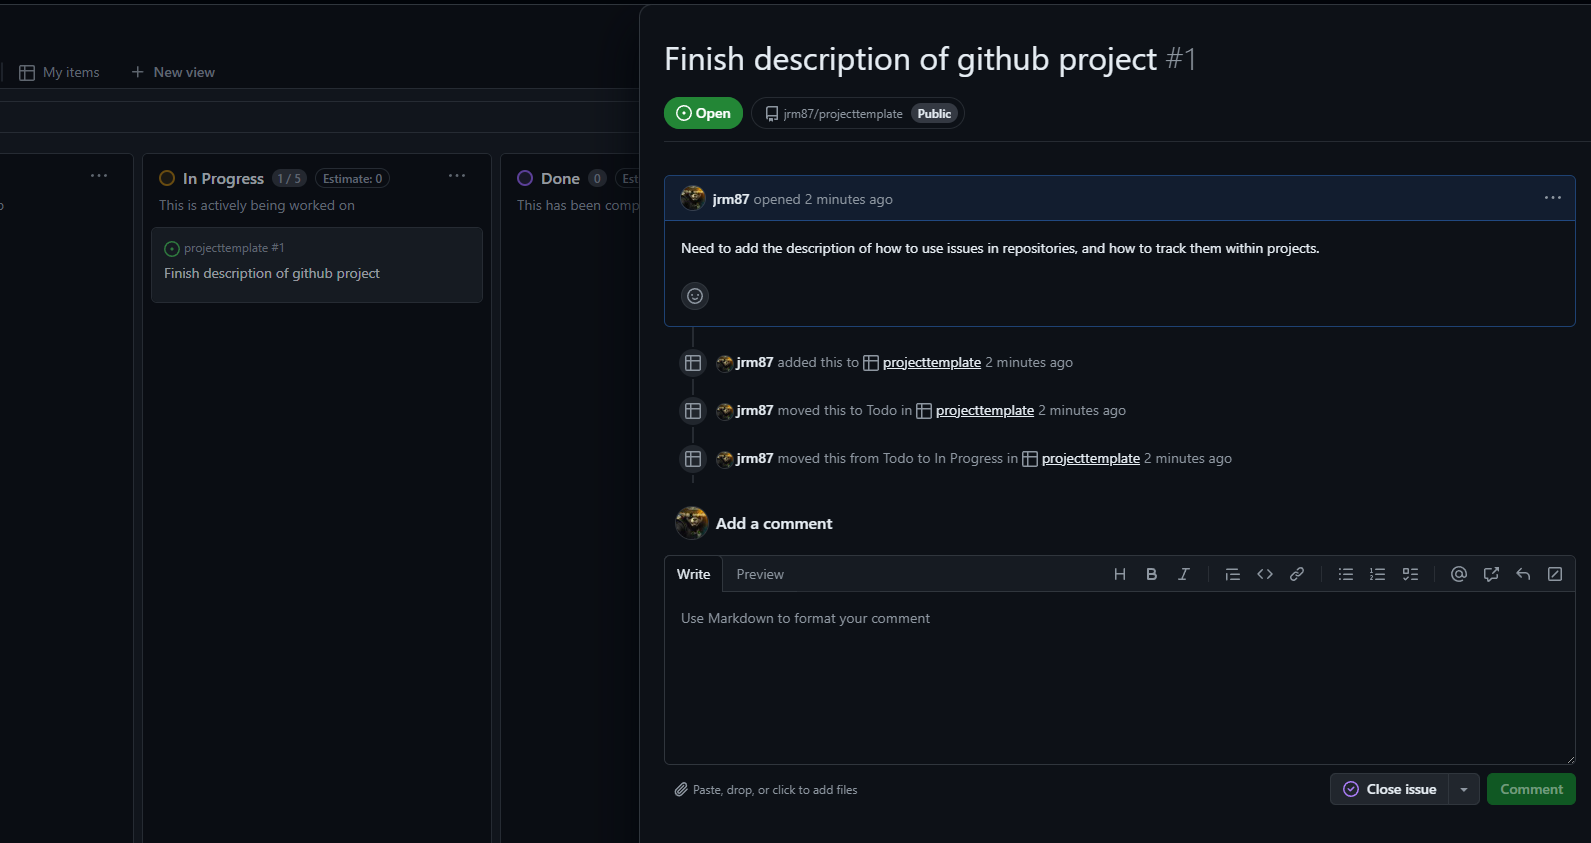
\includegraphics[width=.8\textwidth]{./figures/workflow/gitproject_example3.png}
\end{center}


Note: I have tried using Slack as a project management tool, but I have not enjoyed it.
It is better for free-flowing conversation than keeping a to-do list. 
Asana is very expensive, and my experience with it is fiddly. Thus the current workflow is to use GitHub Projects.